% Summe ca 9 Seiten
\chapter{Ionic 2 Framework}
\label{cha:ionic2}
%
Ionic ist unter Open-Source Lizenz stehendes HTML5 Framework der Firma Drifty, einem unabhängigen Bootstrap-Software Unternehmen, zur Erstellung von Hybrid-Apps. Anfang 2015 wurde die Version 1.0 veröffentlicht, die Version 2.0 steht zum Zeitpunkt der Ausarbeitung dieser Arbeit kurz vor der Veröffentlichung \cite{ionic2Anounce}.
Ionic erweitert Cordova (\fref{sec:ApacheCordova}) um eigene Bibliotheken und verbindet dieses Framework mit AngularJS (\fref{sec:AngularJS}). Ionic unterstützt zudem Syntactically Awesome Style Sheets (SASS) und ist auf die Nutzung mobiler Endgeräte mit Touch-Bedienung optimiert. Ionic liefert eine eigene Bibliothek an Components und Methoden, die den look \& feel einer nativen Applikation schaffen.
%
%
\todo{...}
%
% --------------------------------------------------------------------------------------------
%
\section{Apache Cordova}
\label{sec:ApacheCordova}
%
Das Framework Apache Cordova wurde von der Firma Nitobi entwickelt. Nachdem Nitobi von Adobe Systems aufgekauft wurde hat Adobe Cordova unter dem Namen PhoneGap veröffentlicht und eine Open Source Version unter dem Namen Apache Cordova veröffentlicht \cite{adobePhoneGap}.

Cordova Applikationen bestehen in ihrem Kern aus einer Web-View, in der die Logik der App mittels HTML5, CSS3 und JavaScript realisiert wird. 
Zusätzlich bietet Cordova eine auf Javascript basierende Programmierschnittstelle, die Zugriff auf die nativen Funktionalitäten des Gerätes ermöglicht. So werden mittels APIs Zugriff auf Kamera, Kalender, Adressbuch, GPS-Modul, Dateisystem oder die diversen Sensoren gewährt werden. Diese API ist über Plugins erweiterbar. Persistierung von Datenbankinhalten kann über Local Storage gelöst werden. Es gibt jedoch auch ein Plugin für die Verwendung einer SQLite-Datenbank.

Cordova unterstützt dabei in unterschiedlichem Maße die Plattformen iOS, Android, Blackberry10 und Windows Phone \cite{cordovaSupportedPlatforms}. Android und iOS sind dabei jedoch die am Besten unterstützten Plattformen.

Um die Applikation für die jeweilige Plattform entwickeln zu können wird das native Software Development Kit (SDK) benötigt (Android Studio für Android und XCode für iOS).

Der Strukturelle Aufbau einer Cordova Applikation ist in \fref{fig:Cordovaapparchitecture} dargestellt.
% https://cordova.apache.org/docs/en/latest/guide/overview/index.html 
Die eigentliche Web-Applikation bestehend aus HTML5, JavaScript und CSS-Code wird in einem Ordner namens \emph{www} abgelegt und beim kompilieren in die App kopiert und innerhalb der Cordova App in eine native WebView-Instanz geladen (vgl. \fref{sec:HybrideApplikationen}). In einem eigenen Ordner \emph{Plugins} liegen die nativen Cordova-Plugins, mit deren Hilfe und über eine Javascript-Programmierschnittstelle Zugriff auf native OS-APIs genommen werden kann.
%
% Abbildung Struktureller Aufbau einer Cordova Applikation
\begin{figure}[htb] 
	\centering
	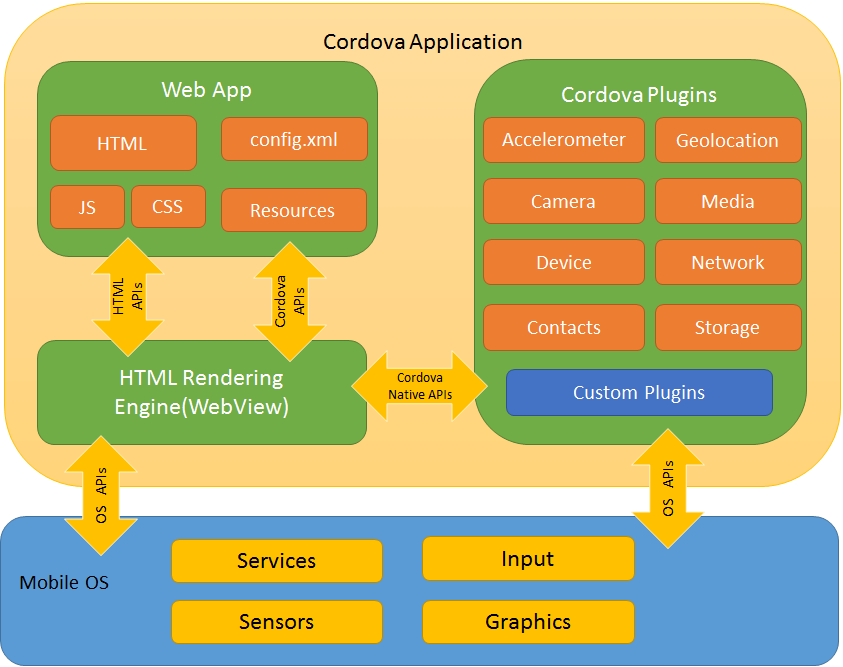
\includegraphics[width=0.6\textwidth]{data/bilder/cordovaapparchitecture.png}
	\caption{Struktureller Aufbau einer Cordova Applikation \cite{cordovaApplicationArchitecture}}
	% https://cordova.apache.org/docs/en/latest/guide/overview/index.html 
	\label{fig:Cordovaapparchitecture}
\end{figure}
%
% --------------------------------------------------------------------------------------------
%
\section{AngularJS}
\label{sec:AngularJS}
%
AngularJS ist ein von Google entwickeltes clientseitiges JavaScript-Framework zur Erstellung von Single-page-Webanwendungen. Es arbeitet dabei nach dem Model-View-ViewModel Entwurfsmuster. AngularJS baut dabei auf der Erweiterung des Vokabulars von HTML auf, um Inhalte der View ohne eine Manipulation des DOM (Document Object Model) mithilfe von JQuery durchführen zu müssen.

Die hier betrachtete Version von AngularJS ist die völlig neugeschriebene Version 2, die auf die Entwicklung mobiler Applikationen ausgelegt ist und auf die Entwicklung mit Typescript ausgelegt ist. Die finale Version von AngularJS 2 wurde im September 2016 veröffentlicht.
%
\subsection{Basiskonzepte von AngularJS 2}
% \cite{DodsonGuideToWebComponents}
% https://css-tricks.com/modular-future-web-components/
AngularJS 2-Projekte sind in Modulen aufgebaut, die je nach Bedarf geladen werden können. Als Basiselement werden sogenannte Components verwendet. Components, also wiederverwendbare JavaScript-Komponenten, sind Klassen, die ein Element in der View repräsentieren. Einer Component wird eine template property zugeordnet und in ihr werden Membervariablen sowie Memberfunktionen gespeichert.

HTML-Templates bilden die View zu einer Component. Mittels Data binding können die Member der Components mit der View verknüpft werden \cite{LynchAngularComponents}. Durch Event binding können Elemente einer View mit Angular-Events (z.B. \texttt{focus}, \texttt{blur} und \texttt{click}) oder selbst definierten Events verbunden werden, die dann Methoden in der jeweiligen Component aufrufen (vgl. auch  \cite{PrechtAngularTemplateSyntax}).

Mithilfe von \emph{structural directives} können direkte DOM-Manipulationen vorgenommen werden. So gibt es Angularspezifische directives wie beispielsweise \texttt{*ngFor}, die wie eine foreach-Schleife einen Container durchlaufen kann und so z.B. schnell eine Tabelle erstellen kann. Ähnlich bedeutend ist die \texttt{*ngIf}-Direktive mit deren Hilfe selektiv an eine Bedingung geknüpft Elemente erzeugt werden können.

\emph{Attribute directives} ändern das Verhalten oder Aussehen bestehender Elemente. So kann beispielsweise mittels der \texttt{ngModel}-Direktive ein two-way-data binding mit einem Attribut einer Component realisiert werden.

Mittels Referenzen auf einzelne Element des DOM können aus einem Element direkt andere Elemente innerhalb der View angesprochen werden.

Services sind Klassen, die wiederverwendbare Funktionalitäten für Components bereitstellen.

Mithilfe des \emph{Dependency injection} Entwurfsmusters werden Components zur Laufzeit mit neuen Instanzen der Services versorgt, die sie benötigen. So werden stets nur die Service-Klassen geladen, die wirklich benötigt werden \cite{angularDocuBasicArchitecture}.
%
% --------------------------------------------------------------------------------------------
%
\section{Konzepte des Ionic 2 Frameworks mit Angular 2}
\label{sec:ionicKonzepte}

Das Ionic-Framework liefert eine große Sammlung an Angular 2-Components die sich frei in ein Cordova-Projekt einbauen lassen. Es liefert zudem verschiedene Styles pro Plattform, die durch komplett verschiedene und unabhängige SASS-Dateien realisiert werden. Eine große über 900 Elemente starke Sammlung an Icons, die sogenannten Ionicons, passt sich zudem dynamisch dem jeweiligen Betriebssystem an und liefert auch so einen möglichst passenden Stil. Ionic Native ist eine Sammlung an Typescript Wrapper für Cordova- bzw. PhoneGap-Plugins die es ermöglichen, grundsätzlich jede Art von nativer Funktionalität zu einer Ionic-App hinzuzufügen \cite{ionic2Docu}.
% https://ionicframework.com/docs/v2/native/
% 
\begin{listing}
    \lstinputlisting{data/sourcecode/ionicExample.html}
    \caption{Beispiel einer typischen \texttt{ion-list}}
    \label{lst:ionicExample}
\end{listing}

Listing \ref{lst:ionicExample} zeigt eine typische View-Implementierung einer Liste mittels der \texttt{ion-list}- und \texttt{ion-item}-Components. Dabei werden mittels der Angular Direktive \texttt{*ngFor} Objekte eines Arrays (hier `songs') aufgelistet. Mittels der in geschweiften Klammern geschriebenen One-Way-Databindings kann auf die Attribute des betrachteten Objektes (hier `\#song') der Schleife zugegriffen werden. Die einzelnen \texttt{ion-item}s werden zudem mit einem Click-Event verknüpft, welches eine in der Component implementierten Methode `openSong' aufruft. Die \texttt{*ngIf} Bedingung sorgt dafür, dass nur bei erfüllter Bedingung das \texttt{<span>}-Element erzeugt wird.
%
% \cite{MoronyAngularAndIonicConcepts} 
% http://www.joshmorony.com/ionic-2-first-look-series-new-angular-2-concepts-syntax/
%
% --------------------------------------------------------------------------------------------
%
\section{Typescriptunterstützung}
%
Die von allen modernen Webbrowsern unterstützte Version von JavaScript ist ES5 (ECMAScript 5), wohingegen die neueste Version ES6 ist. ES6 ist eine Obermenge von ES5 was dazu führt, dass ES5-Code stets auch von ES6 unterstützt wird. Typescript ist eine von Microsoft entwickelte typisierte Version von ES6, deren Verwendung sich für Ionic 2-Projekte anbietet, da Ionic 2 selbst auch in Typescript geschrieben ist und so voll typisiert ist \cite{ionic2Docu}.
%https://ionicframework.com/docs/v2/resources/typescript/

Wird ein Ionic-Projekt über das Ionic CLI (Comand Line Interface) kompiliert, so findet der sogenannte Transpiling-Vorgang in die vom Browser unterstützte ES5 Version statt. Unter Transpiling wird die Umwandlung von Sourcecode zwischen zwei Programmiersprachen verstanden, die einen ähnlichen Abstraktionslevel besitzen, wohingegen Kompilieren allgemein die Übersetzung von einer Programmiersprache (meist einer high-Level Sprache) in eine andere Sprache (meist eine low-Level Sprache) meint. Transpiling ist also eine spezielle Form des Kompilierens. 
\todo{...}
%
% --------------------------------------------------------------------------------------------
%
\section{Struktur eines Ionic2-Projektes}
% https://ionicframework.com/docs/v2/getting-started/tutorial/project-structure/
% http://codingthesmartway.com/ionic-2-project-structure/
\subsection*{./src/}
Innerhalb des src- Ordners liegt der unkompillierte Typescriptcode sowie die Templates. Wird der Buildvorgang per CLI in Gang gesetzt, wird der Code im src- Ordner mittels Transpiling in die korrekte Javascriptversion umgewandelt und in den www-Ordner kopiert.

Im Unterordner \texttt{./src/app/} wird die Haupt-Component der App gespeichert. Diese bildet den Haupteintrittspunkt der App, das sogenannte \emph{root module}.

Im Unterordner \texttt{./src/pages/} werden alle weiteren Pages, also Unterseiten, der App mit ihren Components gespeichert. Jede Page besteht dabei aus einem weiteren Unterordner mit je einer View (html), einer Component (ts) und der zugehörigen Style-Datei (scss).
%
\subsection*{./src/index.html}
In der \texttt{index.html} werden benötigte Scripte und Styles geladen und die eigentliche ionic-App wird mit dem \texttt{<ion-app>}-Tag gestartet. Zudem werden die benötigten Skripte \texttt{cordova.js} und \texttt{build/main.js} geladen.
%
\subsection*{./resources/}
Im Ordner \texttt{resources} liegen die für die App nötigen je nach Plattform typischen Icons und Splashscreens (Startbildschirmbilder). 
%
\subsection*{./assets/}
Im Ordner \texttt{assets} werden ressourcen der App bereitgestellt, die bereits zu Beginn zur Verfügung gestellt werden sollen. So können Datenbanken bereitgestellt werden oder Bilder abgelegt werden.
%